\documentclass{article}
\usepackage[utf8]{inputenc}
\usepackage{hyphenat}
\usepackage{enumitem}
\usepackage{framed}
\usepackage{graphicx}
\usepackage[title,toc,page]{appendix}
\usepackage{arydshln}
\usepackage{hyperref}
\hypersetup{
    colorlinks=true,
    linkcolor=black,
    urlcolor=blue,
    linktoc=all,
    citecolor=black
}

% Coding packages
\usepackage{listings}
\usepackage{lmodern}
\usepackage{xcolor}
\usepackage{algorithm, algpseudocode}
\lstset{
  basicstyle=\ttfamily,
  literate={~} {\raise.17ex\hbox{$\scriptstyle\mathtt{\sim}$}}{1},
  columns=fullflexible,
  frame=single,
  breaklines=true,
  numbers=left,
  stepnumber=1,
  xleftmargin=2em,
  framexleftmargin=1.5em
}

\graphicspath{ {./images/} }

% Referencing
\usepackage[authordate,strict,backend=bibtex8,babel=other,bibencoding=inputenc]{biblatex-chicago}
\addbibresource{references}

% Create the Title 
\title{\large{Curtin University} \\ \large{Curtin Institute of Radio Astronomy} \\ \large{Physics Project 1} \\ \vspace*{20px} \textbf{\LARGE{Finding New Pulsars Using Machine Learning}}\vspace*{10px}}
\author{\vspace*{20px} Jacob Ian Matthews}

\begin{document}


% Build the title page
\begin{titlepage}
    
    \maketitle
    \thispagestyle{empty}
    
    \centering
    \textbf{Supervisors} \\\vspace*{5px}Dr Sam McSweeney and Dr Ramesh Bhat\\

    \vspace*{20px}

    \begin{abstract}

        As radio telescope technology improves, the number of candidate detections to be classified as pulsar or non-pulsar during pulsar surveys increases to the point that it becomes infeasible to classify them manually, a state of affairs known as the ``pulsar candidate selection problem". To solve this problem, machine learning (ML) techniques are used to filter out the non-pulsar candidates in surveys, reducing the number of candidates requiring human evaluation to a manageable number. Here, we adapt an ML solution developed for the LOFAR Tied-Array All-Sky Survey (LOTAAS) for the Southern-sky Murchison Widefield Array Rapid Two-metre (SMART) survey. A group of 147 pulsar and 87 non-pulsar candidates generated by the SMART survey were used to test the LOTAAS ML classifiers trained on a set of 12 pulsar and 13 non-pulsar SMART survey candidates. The classifiers were found, on average, to make accurate pulsar and non-pulsar classifications on SMART survey candidates 87.3\% of the time, compared to the 97.1\% success rate obtained by \textcite{lyon}. Using the machine learning classifiers in ensemble with a selection criteria of three separate positive classifications increased the success rate of non-pulsar classification by 5.2\% (making 0 False Positive classifications), however it decreased the success rate of pulsar classification by 3.5\%. The ensemble machine learning classifier can be further improved by increasing the diversity of pulsars within the machine learning training dataset.

    \end{abstract}



\end{titlepage}

\pagebreak

% Build Table of Contents
\tableofcontents

\pagebreak

% Start sections

% INTRODUCTION SECTION
\section{Introduction}

\subsection{Aim}

This project consists of three aims:
\begin{enumerate}[label=\roman*.]
    \item Investigate the use of Machine Learning (ML) techniques in surveying pulsars;
    \item Create a training dataset for a Machine Learning algorithm to find pulsars in data obtained by the Murchison Widefield Array (MWA); and
    \item Evaluate the utility of the Machine Learning algorithms used by the LOFAR Telescope for the Murchison Widefield Array, and adjust the algorithms as necessary to achieve optimum pulsar candidate classification.
\end{enumerate}

\subsection{Structure of this Report}

In this report, I will first explain in \emph{Section 1.3} how Pulsars, Radio Astronomy, and Machine learning work, and then explain the ``Candidate Selection Problem" \autocite{lyon} and why Machine Learning is necessary in completing future pulsar surveys.

In \emph{Section 2}, I discuss the methods undertaken in: (i) developing the machine learning training dataset for the Murchison Widefield Array, (ii) developing software to validate the output of machine learning classifiers, (iii) evaluating the machine learning algorithms used by the LOFAR surveys for use with the Murchison Widefield Array, and (iv) developing an ensemble machine learning classifier to be used with the Murchison Widefield Array and other radio telescopes.

In \emph{Section 3}, I analyse the results and findings obtained by the methods described in \emph{Section 2}, and in \emph{Section 4} I will discuss (i) the current pulsar classification methods used at the Curtin Institute of Radio Astronomy, (ii) the efficacy of the machine learning classifiers and training dataset produced in this report, and (iii) my concluding remarks about the utility of the machine learning classifiers with the Murchison Widefield Array.

This report will conclude with my recommendations for areas of further development in \emph{Section 5}, and the detailed methodologies in creating the results of this project, and entirety of the source code created undertaking this project, in the \emph{Appendices}.

\pagebreak
\subsection{Background Theory}

\subsubsection{Pulsars}

Pulsars were first detected in 1967 at the Mullard Radio Astronomy Observatory when a periodically pulsing radio source was discovered \autocite{hewish:pulsar}. The pulsing radio source was found to not be man-made or of terrestrial nature, as it could only be observed at a particular declination and right ascension \autocite{hewish:pulsar}. Pulsars were thus suggested to be either rotating white dwarf stars or neutron stars \autocite{hewish:pulsar,gold:pulsar}, the latter suggestion of which was later supported by the works of \textcite{gold:pulsar}. \textcite{gold:pulsar} found that pulsars were more often detected in supernova areas -- supernovae being the producers of neutron stars -- and that pulsars with faster rotations corresponded to younger neutron stars. The theory that a pulsar is a rapidly rotating neutron star was further confirmed by the works of \textcite{ostriker:pulsar}, as well as discovering that pulsars possess a dipole magnetic field that isn't parallel to its rotation axis. A diagram of a pulsar and its magnetic field can be seen in \emph{Figure \ref{fig:pulsar1}}.

\begin{figure}[h!]
    \centering
    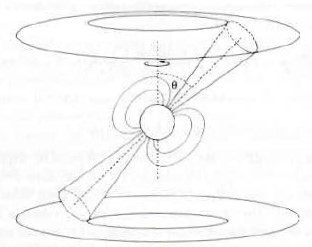
\includegraphics{pulsar.jpg}
    \caption{A pulsar \autocite{maoz}.}
    \label{fig:pulsar1}
\end{figure}

When a star reaches the end of its life, if its initial mass was greater than eight times the mass of the sun, i.e. $8M_{\odot}$, the star will likely supernova, exploding its outer envelope into the surrounding space, leaving the gravitationally collapsed core of the star \autocite{maoz}. This is a neutron star. Using the conservation of angular momentum, we can prove that the collapsed neutron star will have a speed of rotation much greater than the star did prior to the its gravitational collapse. If one considers an ice skater rotating with their arms stretched out, we intuitively know that their speed of rotation will increase if their arms are brought in closer to their body. The same effect applies for a star: if prior to the star's collapse it is rotating at an angular velocity $\omega_1$, the angular velocity $\omega_2$ after the star collapses to a radius of ~11km from a radius thousands of times larger, will be much greater \autocite{maoz}. 

Despite our understanding of the formation of neutron stars and their rotation, the nature of their electromagnetic wave emission is still an active area of research \autocite{lorimer}. The reason that pulsars appear to emit a pulse of radio waves is due to a process called the `lighthouse effect': as the neutron star rotates, the radiated electromagnetic waves sweep across the sky, crossing the line of sight of an observer and producing a pulse-like effect \autocite{lorimer}. When the radio wave passes the line of sight of a radio telescope, the pulse can be recorded. An Integrated Pulse Profile can then be generated from the pulse recorded by the telescope by a process called folding, where a number of separate observations of the pulse can be `stacked' on top of each other to produce a clear representation of the pulse \autocite{helfand:profiles}. An example of an integrated pulse profile can be seen in \emph{Figure \ref{fig:profile}}.

\begin{figure}[h!]
    \centering
    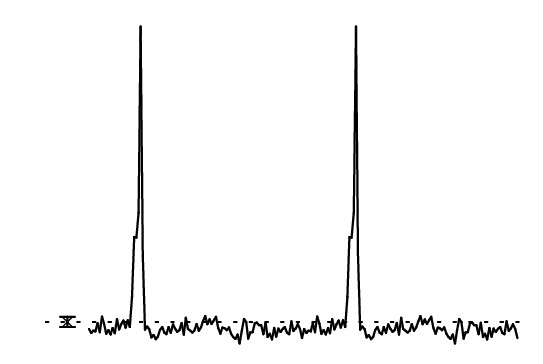
\includegraphics[width=5cm]{PSR_0459-0210-profile.jpg}
    \begin{center}
    \caption{Integrated Pulse Profile of Pulsar 0459-0210 \autocite{swainston:data}.}
    \label{fig:profile}
    \end{center}
\end{figure}

\subsubsection{Sky Surveys}

When completing sky surveys in radio astronomy, it is common to detect many examples of radio frequency interference and noise \autocite{hewish:pulsar,lorimer,lyon,tan}. Radio frequency interference (RFI) is any radio signal that has been unintentionally detected; it normally arises from electrical devices with a periodic nature, such as devices with AC currents, communication systems like radar, or from electrical storms \autocite{lorimer}. Noise, on the other hand, can be detections of the Cosmic Microwave Background (depending on the sensitivity of the radio telescope), or detections of radio waves produced by the electronics of the telescope \autocite{lorimer}. An example of an integrated pulse profile produced by radio frequency interference and noise can be seen in \emph{Figure \ref{fig:rfinoise}}.

\begin{figure}[h!]
    \centering
    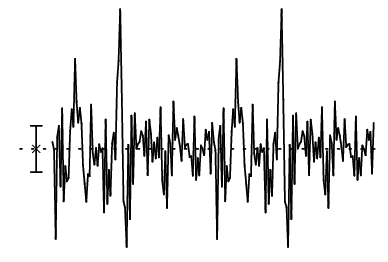
\includegraphics[width=5cm]{rfi.png}
    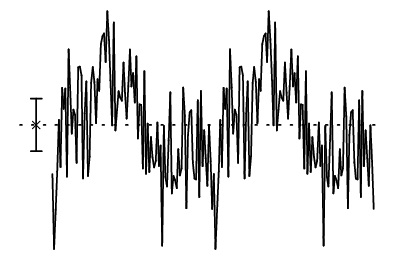
\includegraphics[width=5cm]{noise.png}
    \begin{center}
    \caption{Examples of RFI (left) and Noise (right) \autocite{swainston:data}.}
    \label{fig:rfinoise}
    \end{center}
\end{figure}

It is scientifically important to survey the skies to find new pulsars for a multitude of reasons. For example: due to their extremely reliable periodicity, pulsars can be used as astronomical clocks of high accuracy \autocite{matsakis:pulars}. Also, due to the massive gravitational fields surrounding pulsars, binary pulsars are the definitive area in which to test gravitational theories in the strong-field, such as Einstein's theory of General Relativity, and future research into quantum gravity \autocite{lorimer}.

Throughout the history of pulsar discovery, as the sky survey techniques of detection and radio telescope technology has improved, the number of candidates detected has grown at a very fast rate \autocite{lyon}. The growth rate of the number of candidates stands to increase further with the development of extremely large radio telescopes such as the Square Kilometre Array (SKA) \autocite{lyon}. This introduces a new problem to sky surveying: the candidate selection problem. The candidate selection problem occurs when there are too many detected pulsar candidates to be classified as pulsar or as a non-pulsar than can be feasibly examined by human eyes \autocite{lyon}.

To attempt to solve the candidate selection problem, \textcite{lyon} turned to using a machine learning classifier as an intelligent filter that will filter out the candidates that are radio frequency interference or noise, reducing the candidates to be classified by a human to a more manageable number.

\subsubsection{Machine Learning}

\textcite{valiant} first described machine learning as a function in which a computer completes a task that hasn't been explicitly programmed, it has instead learned to do so. A supervised learning classifier is a function in which a machine learns examples of a particular class and then classifies other inputted data based on the learned model \autocite{dietterich}.

In addressing the candidate selection problem, \textcite{lyon} created a program named \verb|LOTAASClassifier| which contains four separate machine learning algorithms that can be chosen from:
\begin{enumerate}
    \item The C4.5 Decision Tree;
    \item the Multilayered Perceptron;
    \item the Naive Bayes classifier; and
    \item the Support Vector Machine.
\end{enumerate}

The machine learning classifiers from \verb|LOTAASClassifier| generate a classification model from an inputted training dataset, and then they can make classification predictions on the class of pulsar candidates \autocite{lyon}. The training dataset used by \textcite{lyon} contained a set of pulsars, radio frequency interference, and noise. This allows the machine learning classifiers to distinctly identify what is and isn't a pulsar.

By using the machine learning classifiers, \textcite{lyon} was able to accurately predict the class of the candidates 97.1\%. of the time, reducing the number of candidates that had to be manually classified.

\pagebreak
% Methods Section
\section{Methods}
\subsection{Developing the Machine Learning Training Dataset}

Before a machine learning algorithm can make predictions and classify candidates as a pulsar or a non-pulsar, it must first build a classification model from a training dataset which contains similar data with known positive and negative classifications \autocite{tan, lyon}. For the use case of pulsar classification, the training dataset must contain examples of data from both pulsars and from non-pulsars so that the algorithm can learn how to distinguish between the two classes.

To maximise the accuracy of the machine learning algorithm, the input data (including the training dataset) must be composed of a common group of features that can be determined for each candidate that maximises the differences between a pulsar and a non-pulsar. The candidate features used by \textcite{tan} to maximise the differences between pulsar and non-pulsar candidates are:

\begin{equation}
    Prof_{\mu}, Prof_{\sigma}, Prof_{S}, Prof_{k}
\end{equation}

\begin{equation}
    DM_{\mu}, DM_{\sigma}, DM_{S},DM_{k},
    DM_{\mu'}, DM_{\sigma'}, DM_{|S'|},DM_{k'}
\end{equation}

\begin{equation}
    Subband_{\mu}, Subband_{\sigma}, Subband_{S}, Subband_{k}
\end{equation}

\begin{equation}
    Subint_{\mu}, Subint_{\sigma}, Subint_{S}, Subint_{k}
\end{equation}

Where candidate features are calculated from the: (1) Integrated Pulsar Profile, (2) the Dispersion Measure -- Signal-to-Noise Ratio Curve (DM-S/N curve), (3) the correlation coefficients between each sub-band and the integrated pulsar profile, and (4) from the correlation coefficients between each sub-integration and the integrated pulsar profile. 

A set of 12 pulsar and 13 non-pulsar candidates from the SMART survey were provided by N. Swainston to become the machine learning training dataset. The free Python software created by \textcite{lyon}, \verb|PulsarFeatureLab|, was used to process the PRESTO Prepfold \verb|PFD| pulsar candidate files, extracting the above 20 machine learning features from each candidate into a single file of WEKA Data Mining \verb|ARFF| filetype. To create a closed software environment in which the dependencies of the \verb|PulsarFeatureLab| software were unaffected by the host operating system, a containerised virtual operating system was created using the free software Docker (\href{https://docker.com}{https://docker.com}) and the pulsar feature extraction software was thus ran using a bind mounted volume. For further details on how this was achieved, see \emph{Appendix \ref{apndx:pulsarfeaturelab}}.

The file outputted by \verb|PulsarFeatureLab| containing the feature extracted candidates was then edited, removing the `?' character and appending a `1' or `0' to the end of each candidate's line depending on whether the candidate was a pulsar or non-pulsar respectively. This tells the machine learning classifier that candidates with features similar to those preceding the appended binary classification belong to a pulsar (or a non-pulsar). The remaining file constitutes the machine learning training dataset.

\subsection{Developing a Machine Learning Classifier Validation Tool}
\label{sec:methodvalidate}

In order to automate the evaluation of predictions made by the machine learning pulsar classifiers, a Java program named \verb|PulsarValidator| was developed.

\verb|PulsarValidator| was designed to load the positive and negative output files generated from the machine learning classification of a controlled testing dataset of pulsar candidates, and compare these files to a list of the pulsars included in the testing dataset. The software outputs the following statistics: the number of pulsars and non-pulsars, the number of detected pulsars and non-pulsars, and the number of true positives (TP), false positives (FP), true negatives (TN), and false negatives (FN). 

This was achieved by first creating individual Java `ArrayList's to contain the filenames of each candidate found to be a True Positive, False Positive, True Negative, or False Negative classification. The positive and negative output files generated by the classifier (positive denoting pulsars and negative denoting non-pulsars), and the list of pulsars in the testing dataset are then also converted to Java `ArrayList's. The items inside the positive and negative `ArrayList's are then iterated over, checking each item against the list of pulsars. If an item in the positive list is found in the list of pulsars, it is added to the True Positive list, otherwise it is added to the False Positive list. If an item in the negative list is found in the list of pulsars, it is added to the False Negative list, otherwise it is added to the True Negative list. The number of items inside each list is then outputted to the user. This process can be seen in \emph{Algorithm \ref{alg:validator}}. Further details on the development of this software can be found in \emph{Appendix \ref{apndx:pulsarvalidator}}, and the full Java source code can be found in \emph{Appendix \ref{src:pulsarvalidator}} or on GitHub (\href{https://github.com/jacob-ian/PulsarValidator.git}{https://github.com/jacob-ian/PulsarValidator.git}).

\begin{algorithm}
    \caption{Pulsar Validator (pseudocode)}
    \label{alg:validator}
    \begin{algorithmic}
        \State Let $truePositive$ = new List
        \State Let $falsePositive$ = new List
        \State Let $trueNegative$ = new List
        \State Let $falseNegative$ = new List
        
        \For{each $item$ in $classifierPositive$ list}
            \State Let Boolean $found$ = false
            \State Let Integer $i=0$
            \While{$found$ is false}
                \If{$i$th item in $pulsarList$ is $item$}
                    \State add $item$ to $truePositive$ list
                    \State $found$ = true
                \ElsIf{$i$ equals number of items in $pulsarList$}
                    \State add $item$ to $falsePositive$ list
                    \State $found$ = true
                \Else
                    \State $i$=$i+1$
                \EndIf
            \EndWhile
        \EndFor

        \For{each $item$ in $classifierNegative$ list}
            \State Let Boolean $found$ = false
            \State Let Integer $i=0$
            \While{$found$ is false}
                \If{$i$th item in $pulsarList$ is $item$}
                    \State add $item$ to $falseNegative$ list
                    \State $found$ = true
                \ElsIf{$i$ equals number of items in $pulsarList$}
                    \State add $item$ to $truePositive$ list
                    \State $found$ = true
                \Else
                    \State $i$=$i+1$
                \EndIf
            \EndWhile
        \EndFor
        \State Let $TP$ = number of items in $truePositive$
        \State Let $TN$ = number of items in $trueNegative$
        \State Let $FP$ = number of items in $falsePositive$
        \State Let $FN$ = number of items in $falseNegative$
        \State Let $Pulsars$ = $TP+FN$
        \State Let $NonPulsars$ = $TN+FP$
        \State Output $Pulsars$, $NonPulsars$, $TP$, $FP$, $TN$, $FN$
    \end{algorithmic}
\end{algorithm}

\subsection{Developing an Ensemble Machine Learning Classifier}

To implement the ensemble classifier feature outlined by \textcite{tan} to the \verb|LOTAASClassifier| software, a new Java program named \verb|PulsarClassifier| was developed.

\verb|PulsarClassifier| was designed so that a new `ensemble classifier' option can be chosen as the classification algorithm as well as the previously existing algorithms from \verb|LOTAASClassifier|. The program outputs the classification results of all machine learning classifiers from the \verb|LOTAASClassifier| program, as well as that of the new ensemble classifier. This was achieved by creating the following new Java classes: `PulsarClassifier', `ClassPredictor', `ClassifierBuilder', and `ClassifierValidator', and extending the existing versions of those classes from \verb|LOTAASClassifier| to maintain some of the prior methods and properties.

The Java classes `ClassifierBuilder' and `ClassifierValidator' were modified such that if the user selected the ensemble classifier as the classification algorithm, the method involved in building or validating a machine learning classifier would iterate through the list of available machine learning classifiers (C4.5, Multi-Layered Perceptron, Naïve Bayes, and Support Vector Machine) to build a classification model for each ML classifier, or validate each ML classifier, respectively. These processes can be seen in \emph{Algorithm \ref{alg:classifierbuilder}} and \emph{Algorithm \ref{alg:classifiervalidator}}.

\begin{algorithm}[H]
    \caption{ClassifierBuilder (pseudocode)}
    \label{alg:classifierbuilder}
    \begin{algorithmic}[1]
        \If{$algorithm = -1$}
            \For{each algorithm $i=1\rightarrow 4$}
                \Comment Loop through all classifiers
                \State buildClassifier($i$, $trainingSet$, $modelsDirectory$)
            \EndFor
        \Else 
            \Comment Build individual classifier
            \State buildClassifier($algorithm$, $trainingSet$, $modelPath$)
            
        \EndIf
    \end{algorithmic}
\end{algorithm}

\begin{algorithm}[H]
    \caption{ClassifierValidator (pseudocode)}
    \label{alg:classifiervalidator}
    \begin{algorithmic}[1]
        \If{$algorithm = -1$}
            \For{each algorithm $i=1\rightarrow 4$}
                \Comment Loop through all classifiers
                \State testClassifier($i$, $testSet$, $modelsDirectory$)
            \EndFor
        \Else 
            \Comment Test individual classifier
            \State testClassifier($algorithm$, $testSet$, $modelPath$)
        \EndIf
        
    \end{algorithmic}
\end{algorithm}

The Java class `ClassPredictor' was modified such that if the user chooses to use the ensemble classifier, a Java `ArrayList' is created to store the filepaths to the outputs of each machine learning classifier. The list of available machine learning classifiers is then iterated over, generating the classification predictions from each classifier and adding their outputs to the created list of output files. The Java classes `Classification' and `ClassificationList' are then created to be a key-value pair data class and a list of key-value classifications respectively, where the key denotes the filename of a candidate and the value denotes the number of times this candidate has been given a particular classification. A `ClassificationList' for positive and negative classifications are then constructed and the candidates in the positive and negative classifier output files are iterated over, adding the candidates to their respective lists and incrementing their associated value for every recurring classification. As discussed in \textcite{tan}, a positive classification in an ensemble classifier is generally made when a candidate has received a positive classification from 3 separate classifiers. To implement this selection criteria, the positive `ClassificationList' is iterated over and the candidates with an associated value less than 3 are moved into the negative `ClassificationList'. The remaining positive and negative `ClassificationList's are then outputted to their respective positive and negative output files for the ensemble classifier. This process can be seen in \emph{Algorithm \ref{alg:classpredictor}}.

\begin{algorithm}
    \caption{ClassPredictor (pseudocode)}
    \label{alg:classpredictor}
    \begin{algorithmic}[1]
        \If{$algorithm = -1$}
            \State list = new OutputFileList()
            \For{algorithm $i=1\rightarrow4$}
                \Comment Loop through all classifiers
                \State makePredictions($i$, $inputData$, $modelsDirectory$)
                \State list.add(ClassifierOutputFiles)
                \Comment Add output filepaths to list
            \EndFor
            \State positiveList = new ClassificationsList()
            \State negativeList = new ClassificationsList()
            \Comment Create classification lists
            \For{each OutputFile from list}
                \If{OutputFile is .positive}
                    \For{each line in OutputFile}
                        \State positiveList.add(line)
                        \Comment Add to +ve classifications
                    \EndFor
                \ElsIf{OutputFile is .negative}
                    \For{each line in OutputFile}
                        \State negativeList.add(line)
                        \Comment Add to -ve classifications
                    \EndFor
                \EndIf
            \EndFor
            \For{each classification in positiveList}
                \If{classification.occurrences $< 3$}
                    \State negativeList.add(classification)
                    \Comment cut-off at $< 3$ classifications
                \Else
                    \State positiveOutput(classification)
                    \Comment Output classified as Pulsar
                \EndIf
            \EndFor
            \For{each classification in negativeList}
                \State negativeOutput(classification)
                \Comment Output classified as non-Pulsar
            \EndFor

        \Else 
            \State makePredictions($algorithm$)
            \Comment Use individual classifier
        \EndIf
    \end{algorithmic}
\end{algorithm}

The final modification that was made included changing the Java class `PulsarClassifier' to include the ensemble classifier as an option in the user selectable algorithms. Further details on the development of this software can be found in \emph{Appendix \ref{apndx:pulsarclassifier}} and the full Java source code can be found in \emph{Appendix \ref{src:pulsarclassifier}} or on GitHub (\href{https://github.com/jacob-ian/PulsarClassifier.git}{https://github.com/jacob-ian/PulsarClassifier.git}).

\subsection{Evaluating the Machine Learning Classifiers}

A set of 147 pulsar and 87 non-pulsar candidates generated by the SMART survey were then provided by N. Swainston to test the machine learning classifiers on Murchison Widefield Array data. To test all machine learning classifiers present in \verb|LOTAASClassifier|, and the ensemble classifier, the new \\\verb|PulsarClassifier| program was used.

Before making predictions on the test data, it is necessary to create the machine learning classification models from the training dataset. Using \\\verb|PulsarClassifier|, the training dataset was used to generate the classification models for each ML classifier. \verb|PulsarFeatureLab| was then used to extract the machine learning features from the testing dataset of candidates. \verb|PulsarClassifier| was then used to classify the candidates in the testing dataset with the ensemble classifier (and hence with each of the other ML classifiers). For details on the use of \verb|PulsarClassifier|, see \emph{Appendix \ref{apndx:usepulsarclassifier}}.

To evaluate the accuracy of the predictions of the machine learning classifiers, a list of the pulsars included in the testing dataset was created and \verb|PulsarValidator| was ran with the output files of each classifier. For details on the use of \verb|PulsarValidator|, see \emph{Appendix \ref{apndx:usepulsarvalidator}}.

\pagebreak
% Results Section
\section{Results and Analyses}
\subsection{Machine Learning Training Dataset}

The machine learning training dataset created with candidates detected by the Murchison Widefield Array can be found under \emph{Appendix \ref{sec:training}}.

\subsection{Classification Results from the LOTAASClassifier Algorithms}

\subsubsection{The J48 Algorithm}

The output created by \verb|PulsarValidator| on analysis of the classification results of the J48 (C4.5 Decision Tree) algorithm is as follows:

\begin{lstlisting}[numbers=none]
Number of Pulsars: 147
Pulsars Detected: 146
True Positives: 131
False Positives: 15

Number of Non-Pulsars: 87
Non-Pulsars Detected: 88
True Negatives: 72
False Negatives: 16
\end{lstlisting}

We can therefore calculate the pulsar classification success rate to be:

$$ R_{p} = \frac{TP}{N_p} = \frac{131}{147} =  0.8911 = 89.11\%,$$

where $N_p$ is the number of pulsars in the testing dataset and $TP$ is the number of true positive classifications. The non-pulsar classification success rate can be found as:

$$R_{np} = \frac{TN}{N_{np}} = \frac{72}{87} = 0.8275 = 82.75\%,$$

where $N_{np}$ is the number of non-pulsars in the testing dataset and $TN$ is the number of true negative classifications.

\subsubsection{The Multi-Layer Perceptron Algorithm}

The output created by \verb|PulsarValidator| on analysis of the classification results of the Multi-Layer Perceptron algorithm is as follows:

\begin{lstlisting}[numbers=none]
Number of Pulsars: 147
Pulsars Detected: 125
True Positives: 123
False Positives: 2

Number of Non-Pulsars: 87
Non-Pulsars Detected: 109
True Negatives: 85
False Negatives: 24
\end{lstlisting}

We can therefore calculate the pulsar classification success rate to be:

$$ R_{p} = \frac{TP}{N} = \frac{123}{147} =  0.8367 = 83.67\%,$$

where $N$ is the number of pulsars in the testing dataset, and $TP$ is the number of true positive classifications. The non-pulsar classification success rate can be found as:

$$R_{np} = \frac{TN}{N_{np}} = \frac{85}{87} = 0.9770 = 97.70\%,$$

where $N_{np}$ is the number of non-pulsars in the testing dataset and $TN$ is the number of true negative classifications.

\subsubsection{The Naïve Bayes Tester Algorithm}

The output created by \verb|PulsarValidator| on analysis of the classification results of the Naïve Bayes algorithm is as follows:

\begin{lstlisting}[numbers=none]
Number of Pulsars: 147
Pulsars Detected: 119
True Positives: 118
False Positives: 1

Number of Non-Pulsars: 87
Non-Pulsars Detected: 115
True Negatives: 86
False Negatives: 29
\end{lstlisting}

We can therefore calculate the pulsar classification success rate to be:

$$ R_{p} = \frac{TP}{N} = \frac{118}{147} =  0.8027 = 80.27\%,$$

where $N$ is the number of pulsars in the testing dataset, and $TP$ is the number of true positive classifications. The non-pulsar classification success rate can be found as:

$$R_{np} = \frac{TN}{N_{np}} = \frac{86}{87} = 0.9885 = 98.85\%,$$

where $N_{np}$ is the number of non-pulsars in the testing dataset and $TN$ is the number of true negative classifications.

\subsubsection{The Support Vector Machine Algorithm}

The output created by \verb|PulsarValidator| on analysis of the classification results of the Naïve Bayes algorithm is as follows:

\begin{lstlisting}[numbers=none]
Number of Pulsars: 147
Pulsars Detected: 97
True Positives: 97
False Positives: 0

Number of Non-Pulsars: 87
Non-Pulsars Detected: 137
True Negatives: 87
False Negatives: 50
\end{lstlisting}

We can therefore calculate the pulsar classification success rate to be:

$$ R_{p} = \frac{TP}{N} = \frac{97}{147} =  0.6598 = 65.98\%,$$

where $N$ is the number of pulsars in the testing dataset, and $TP$ is the number of true positive classifications. The non-pulsar classification success rate can be found as:

$$R_{np} = \frac{TN}{N_{np}} = \frac{87}{87} = 1.00 = 100.00\%,$$

where $N_{np}$ is the number of non-pulsars in the testing dataset and $TN$ is the number of true negative classifications.

\subsection{Classification Results from the PulsarClassifier Ensemble Classifier}

The output created by \verb|PulsarValidator| on analysis of the classification results of the \verb|PulsarClassifier| ensemble classifier is as follows:

\begin{lstlisting}[numbers=none]
Number of Pulsars: 147
Pulsars Detected: 112
True Positives: 112
False Positives: 0

Number of Non-Pulsars: 87
Non-Pulsars Detected: 122
True Negatives: 87
False Negatives: 35
\end{lstlisting}

We can therefore calculate the pulsar classification success rate to be:

$$ R_{p} = \frac{TP}{N} = \frac{112}{147} =  0.7619 = 76.19\%,$$

where $N$ is the number of pulsars in the testing dataset, and $TP$ is the number of true positive classifications. The non-pulsar classification success rate can be found as:

$$R_{np} = \frac{TN}{N_{np}} = \frac{87}{87} = 1.00 = 100.00\%,$$

where $N_{np}$ is the number of non-pulsars in the testing dataset and $TN$ is the number of true negative classifications.

\subsection{Compilation of Results and Analyses}

A table containing the number of true and false positives and negatives for each classifier can be found below in \emph{Table \ref{tab:compiled}}:

\begin{table}[H]
    \centering
    
    \caption{Compiled Results of the Machine Learning Classifiers}

    \begin{framed}
        \begin{tabular}{l c c c c}
            & \multicolumn{2}{c}{Pulsars} & \multicolumn{2}{c}{Non-Pulsars} \\
            Classifier & TP & FN & TN & FP \\
            \hline
            \hline
            LOTAASClassifier &  &  & \\
            \hline
            J48 & 131 & 16 & 72 & 15 \\
            MLP & 123 & 24 & 85 & 2 \\
            NB & 118 & 29 & 86 & 1 \\
            SVM & 97 & 50 & 87 & 0 \\
            \hline
            PulsarClassifier &  &  & \\
            \hline
            Ensemble & 112 & 35 & 87 & 0 \\
            \hline
            \hline
        \end{tabular}

        \vspace{8px}
        TP: Number of True Positives.\\
        FN: Number of False Negatives.\\
        TN: Number of True Negatives.\\
        FP: Number of False Positives. \\
    \end{framed}
    \label{tab:compiled}
\end{table}

A table containing the pulsar and non-pulsar classification success rates of all algorithms and the ensemble classifier can be found below in \emph{Table \ref{tab:analyses}}:

\begin{table}[H]
    \centering
    
    \caption{Success Rates of Each Pulsar Classifier}

    \begin{framed}
        \begin{tabular}{l c c c}
            Classifier & $R_p$ & $R_{np}$ & $Combined$ \\
            \hline
            \hline
            LOTAASClassifier &  &  & \\
            \hline
            J48 & 89.11\% & 82.75\% & 85.93\% \\
            MLP & 83.67\% & 97.70\% & 90.69\% \\
            NB & 80.27\% & 98.85\% & 89.56\%\\
            SVM & 65.98\% & 100.00\% & 82.99\% \\
            \hdashline 
            \emph{Average} & 79.76\% & 94.83\% & 87.30\% \\
            \hline
            PulsarClassifier &  &  & \\
            \hline
            Ensemble & 76.19\% & 100.00\% & 88.10\% \\
            \hline
            \hline
        \end{tabular}

        \vspace{8px}
        $R_p$: Success rate of pulsar classification.\\
        $R_{np}$: Success rate of non-pulsar classification. \\
        $Combined$: Combined success rate (total accuracy).\\
    \end{framed}
    \label{tab:analyses}
\end{table}

\pagebreak
% Results Discussion Section
\section{Discussion and Conclusions}
\subsection{Evaluating Curtin Institute of Radio Astronomy's Pulsar Classification Pipeline}

A pulsar classification pipeline can be defined as the process undertaken to classify a candidate as a pulsar \autocite{swainston}. The current pipeline at the Curtin Institute of Radio Astronomy (CIRA) for pulsar classification is as follows:
\begin{enumerate}[label=\roman*.]
    \item Generate pulsar candidates through the SMART (Southern-sky MWA Rapid Two-metre) survey;
    \item Extract machine learning features from the pulsar candidates using \\\verb|PulsarFeatureLab|;
    \item Use the LOFAR Tied-Array All-Sky machine learning pulsar classifier, \verb|LOTAASClassifier|, to to eliminate a large number of pulsar candidates; and
    \item Manually inspect the remaining pulsar candidates to confirm pulsar discovery.
\end{enumerate}
\autocite{swainston:git}. While the classification pipeline itself appears to be optimal, I have identified a few issues with the previous attempts at CIRA in using the machine learning classifier.

The first issue revolves around the use of mislabelled and incomplete software. In the research completed by \textcite{tan}, the original \\\verb|LOTAASClassifier|, created by \textcite{lyon}, was upgraded to include two major new features: (i) ensemble classification, and (ii) radio frequency interference (RFI) classification. The machine learning feature set was also expanded from 8 features in \textcite{lyon} to 20 features in \textcite{tan}, greatly improving the accuracy of classification. Upon analysis of the source code of \verb|LOTAASClassifier|, it appears that the two new classification features were not released publicly, despite the software being labelled as \verb|LOTAASClassifier v2.0| in its main Java class, the same name referenced by \textcite{tan}. Despite this, the new, expanded set of machine learning features was released with \verb|PulsarFeatureLab Version 1.3.2|. This created a mismatch between the feature extraction software and the machine learning classifier, which leads to the next issue in the CIRA pipeline: the training dataset.

In the pipeline provided by \textcite{swainston:git}, it appears that CIRA has been attempting to use the training dataset generated for the LOFAR Tied-Array All-Sky Survey included with the \verb|LOTAASClassifier| software, for pulsar candidates generated in the SMART survey. In itself, this may not present issues, however due to the unknown mismatch in the machine learning software, an issue of feature dimensions occurs. The included training dataset creates a classification model with the original 8 machine learning features, therefore any predictions on new candidates would require the same 8 machine learning features to have been extracted prior to classification. Due to the mislabelled software, CIRA has been extracting the set of 20 features from pulsar candidates and attempting to make classifications against a set of 8 features, preventing classifications from occurring in \verb|LOTAASClassifier| due to a mismatch in dimensions. This issue can be fixed by creating a training dataset with the same set of extracted features as will be present in the candidates for classification.

The final issue arising in the CIRA pipeline also spouts from the mislabelling of the \verb|LOTAASClassifier| software. The CIRA pipeline expects that the ensemble classifier created in the upgraded software from \textcite{tan} will be used. Without the latest version of \verb|LOTAASClassifier| having been released, the CIRA pipeline defaults to using the J48 machine learning classification algorithm. As seen in Table \ref{tab:analyses} from \emph{Section 3.4}, the J48 algorithm does not appear to be optimal in combined pulsar and non-pulsar classification. To fix this issue, an ensemble machine learning classifier was created in \emph{Section 2.3} to replace the \verb|LOTAASClassifier| software.

\subsection{Evaluating the Training Dataset and Machine Learning Classifiers}

An evaluation of the machine learning classifiers: \verb|LOTAASClassifier| and its algorithms, and \verb|PulsarClassfier|, will in its nature be subject to the quality of the training dataset used. By inspecting the data produced in \emph{Section 3.2}, we can see the success rates of pulsar and non-pulsar classification, which are defined as the ratio of the number of true positive (true negative) classifications with the number of pulsars (non-pulsars). The success rates of each classifier are then compiled into Table \ref{tab:analyses}. Another metric, the combined success rate, is also introduced as the mean of the two success rates. The combined success rate can be used to rank the total accuracy of the classifiers, however this metric does not contain ample information. The classifiers can thus be ranked in order of highest total accuracy:

\begin{enumerate}
    \item Multi-Layered Perceptron (90.69\%)
    \item Naïve Bayes Test (89.56\%)
    \item Ensemble Classifier (88.10\%)
    \item J48 (C4.5 Decision Tree) (85.93\%)
    \item Support Vector Machine (82.99\%)
\end{enumerate}

Despite being ranked third in combined success rates, the \verb|PulsarClassifier|'s Ensemble Classifier was only one of two classifiers that correctly classified all examples of noise and radio frequency interference as \emph{non-pulsar}, the other successful classifier being the Support Vector Machine. As a result of this, there were no false positive classifications completed by the Ensemble classifier, i.e. everything classified as a pulsar actually was a pulsar. The Ensemble Classifier was let down by misclassifying 35 pulsars, having the second-lowest success rate of pulsar classification - the lowest being the Support Vector Machine which misclassified 50 pulsars, and the highest being the J48 Classifier having misclassified only 16 pulsars. 

For the use case of classifying pulsar candidates generated from the Murchison Widefield Array, the most important metric to be considered when evaluating a machine learning classifier is the pulsar classification success rate. It is more important to not miss the classification of a pulsar and less important if a non-pulsar is classified as a pulsar. For this reason, the objective is to maximise the rate of true positive classifications and minimise the rate of false negative classifications.

The training dataset created in this project contained 11 examples of pulsars and 12 examples of noise and radio frequency interference (RFI). While the training dataset appeared to have a satisfactory variety of noise and RFI, contributing to the ensemble classifier's perfect rate of non-pulsar classification, the set of pulsars appeared to be unsatisfactory. In order to improve the success rate of pulsar classification (positive success rate) in the ensemble classifier, we must use a modified training dataset that will improve the positive success rate in the worst performing individual classifiers: the Support Vector Machine (65.98\%), and the Naïve Bayes Test (80.27\%), whilst maintaining the higher positive success rates of the other classifiers. By doing so, more pulsars will survive the ensemble classifier's individual classification criteria of 3 or more, and thus the positive success rate will improve. This modification to the training dataset could involve changing the included set of pulsars to include a subset of pulsars of ordinary appearing features, and the remaining subset of pulsars should exhibit unusual or difficult to discern features.

In conclusion, I believe that the machine learning classifiers in the \\\verb|LOTAASClassifier| software, particularly used in ensemble such as with the \verb|PulsarClassifier| software created for this project, are of great utility for current and future Murchison Widefield Array pulsar surveys. As discussed in \textcite{lyon}, the number of pulsar candidates generated in pulsar surveys stands to grow exponentially beyond the economical capacity of data storage and viability of manual examination. This problem requires a solution to filter out the non-pulsars from the group of candidates to maximise the discovery of pulsars, and I believe that the \verb|PulsarClassifier| software is another step forward in solving the problem. While the training dataset does require further development to maximise the success of the Ensemble Classifier, the Machine Learning techniques themselves proved to be extremely valuable in pulsar classification.


\pagebreak
% RECOMMENDATIONS SECTION
\section{Recommendations}

For further development of the Machine Learning classifiers and strategies used in this project, I would recommend undertaking the following tasks:

\begin{enumerate}
    \item Investigate and fix the Python \verb|Traceback Error| produced by the software \verb|PulsarFeatureLab v1.3.2|:

    During the usage of this feature extraction software, some \verb|PFD| candidate files would cause a \verb|Traceback| error to be produced, causing the feature extraction to fail for that particular candidate. The result of these failures was that there was a smaller dataset to train the machine learning classifiers on, and a smaller dataset to make machine learning classification predictions on.

    \item Build the Radio Frequency Interference (RFI) classification feature discussed by \textcite{tan} into \verb|PulsarClassifier|:
    
    According to \textcite{tan}, by also including the classification category of RFI, the accuracy of the machine learning ensemble classifier was increased. The result of this feature would be three classifier output files: \verb|output.pulsars|, \verb|output.rfi|, and \verb|output.other|.

    \item Use a more diverse Training Dataset:

    Due to constraints on the available \verb|PFD| candidate data during this project, I was unable to use a large set of pulsar and non-pulsar candidates in the training dataset. By using a training dataset that is more diverse, the \verb|PulsarClassifier| will be more accurate in its predictions.
\end{enumerate}

\pagebreak
% REFERENCES SECTION
\section{References}
\printbibliography[heading=none]

\pagebreak
% APPENDICES SECTION
\begin{appendices}

    \section{Methods}
    \begin{subappendices}
        \subsection{Feature Extraction with PulsarFeatureLab}
        \label{apndx:pulsarfeaturelab}

        First, a directory to store the Dockerfile and pulsar candidate data is created by completing the following commands in a UNIX terminal:

        \begin{lstlisting}[numbers=none]
$ mkdir ~/pulsars
$ cd ~/pulsars
$ touch Dockerfile
        \end{lstlisting}

        To create the Docker image, the contents of the \verb|Dockerfile| can be edited to contain:

        \begin{lstlisting}[title=Dockerfile]
FROM alpine/git:latest as builder
WORKDIR /root/
RUN cd /root/ && git clone --single-branch --branch V1.3.2 https://github.com/scienceguyrob/PulsarFeatureLab.git && mkdir PulsarFeatureLab/PulsarFeatureLab/Data/IO

FROM python:2.7
WORKDIR /usr/src/app
COPY --from=builder /root/PulsarFeatureLab .
RUN pip install numpy scipy matplotlib astropy
ENTRYPOINT ["python", "./PulsarFeatureLab/Src/PulsarFeatureLab.py"]
        \end{lstlisting}

        The above \verb|Dockerfile| instructs Docker to:
        \begin{enumerate}[label=\roman*.]
            \item use an image of Alpine Linux with \verb|git| preinstalled to download the \verb|PulsarFeatureLab| software from GitHub \\(https://github.com/scienceguyrob/PulsarFeatureLab);
            \item create a directory inside the downloaded software to store the input and output data;
            \item create a Docker image based on Python 2.7;
            \item transfer the \verb|PulsarFeatureLab| software into the Python 2.7 image; and
            \item install \verb|PulsarFeatureLab|'s library dependencies (\verb|NumPy, SciPy, matplotlib| and \verb|astropy|).
        \end{enumerate}

        The above Docker image can now be built into a container (a virtual operating system) and a directory to hold the input data can be created by running the following commands on a UNIX terminal:

        \begin{lstlisting}[numbers=none]
$ docker build -t jacobianm/pulsarfeaturelab:1.3.2 .
$ mkdir ~/pulsars/data/pfd
        \end{lstlisting}

        For future development of this project, the Docker image \\\verb|jacobianm/pulsarfeaturelab:1.3.2| is available on Docker Hub\\(https://hub.docker.com) and will be automatically downloaded when running the \verb|docker run| command below. Candidate \verb|PFD| files of known pulsars and non-pulsars detected by the Murchison Widefield Array (MWA) can now populate the above created directory, and the following command can be ran to extract the features from the candidates:

        \begin{lstlisting}[numbers=none]
$ docker run --rm -v ~/pulsars/data/pfd:/usr/src/app/PulsarFeatureLab/Data/IO jacobianm/pulsarfeaturelab:1.3.2 -d "/usr/src/app/PulsarFeatureLab/Data/IO" -c 3 -t 6 -f "/usr/src/app/PulsarFeatureLab/Data/IO/output.arff" --arff --meta
        \end{lstlisting}

        This function instructs Docker to connect the directory containing the \verb|PFD| files to the \verb|PulsarFeatureLab| container's input/output directory and then run the \verb|PulsarFeatureLab| software with arguments stating where the input files are, what filetype they are (\verb|PFD|), which set of features to extract, and where to place the output file (\verb|output.arff|).

        \subsection{Developing PulsarValidator}
        \label{apndx:pulsarvalidator}
        We begin by creating a new Java project using the free software Maven (https://maven.apache.org) by running the following commands in a UNIX terminal:

        \begin{lstlisting}[numbers=none]
$ cd ~/pulsars
$ mkdir PulsarValidator && cd PulsarValidator
$ mvn archetype:generate -DarchetypeGroupId=org.apache.maven.archetypes -DarchetypeArtifactId=maven-archetype-quickstart -DarchetypeVersion=1.4
        \end{lstlisting}
        
        We can then create the following file structure and resynchronise the project:
        
        \begin{lstlisting}[numbers=none]
PulsarValidator/
    src/
        main/
            java/
                com/jacobianmatthews/pulsarvalidator/
                    PulsarValidator.java
        test/
            ...
    target/
            ...
    pom.xml
        \end{lstlisting}
        
        The file: \verb|PulsarValidator.java| stands as the entry-point to the software and will be compiled into an executable \verb|JAR| file upon completion of creating the software.
        
        This software will process a user inputted \verb|String| containing the path to a file with the list of pulsars included in the dataset classified by the machine learning classifier, a user inputted \verb|String| containing the path to the \verb|.positive| file created by the classifier, and a user inputted \verb|String| containing the path to the \verb|.negative| file created by the classifier\footnote{The '.positive' file contains the candidates classified as pulsars, and the '.negative' file contains the candidates classified as non-pulsars.}. These will be inputted as command-line arguments when the user runs the Java executable file.
        
        To access the user inputted arguments, we can include the following function in the \verb|main(String[] args)| method of the \verb|PulsarValidator.java| class:
        
        \begin{algorithm}[H]
            \caption{getCliVariables(args) (pseudocode)}
            \begin{algorithmic}
                \For{Integer $i=0\rightarrow$ number of arguments in $args$}
                    \If{$i$th argument in $args$ is "-v"}
                        \State Let Boolean $ValidationMode$ = true
                        \State Let String $pulsarListPath$ = ($i+1$)th argument in $args$
                        \State Let String $classifierPositive$ = ($i+2$)th argument in $args$
                        \State Let String $classifierNegative$ = ($i+3$)th argument in $args$
                    \EndIf
                \EndFor
            \end{algorithmic}
        \end{algorithm}
        
        We can then use a simple conditional statement after this function is ran to check if the \verb|Boolean ValidationMode| has been set to \verb|true|, to determine whether to continue the validation. The complete Java class \verb|PulsarValidator.java| can be seen in \emph{Appendix \ref{src:pulsarvalidator:entry}}.
        
        We can then create a new Java class, \verb|ValidationMode.java|, with the following algorithm to validate the output of the classifier against the list of pulsars:
        
        \begin{algorithm}[H]
            \caption{ValidationMode.java (pseudocode)}
            \begin{algorithmic}
                \State Let $truePositive$ = new List
                \State Let $falsePositive$ = new List
                \State Let $trueNegative$ = new List
                \State Let $falseNegative$ = new List
                
                \For{each $item$ in $classifierPositive$ list}
                    \State Let Boolean $found$ = false
                    \State Let Integer $i=0$
                    \While{$found$ is false}
                        \If{$i$th item in $pulsarList$ is $item$}
                            \State add $item$ to $truePositive$ list
                            \State $found$ = true
                        \ElsIf{$i$ equals number of items in $pulsarList$}
                            \State add $item$ to $falsePositive$ list
                            \State $found$ = true
                        \Else
                            \State $i$=$i+1$
                        \EndIf
                    \EndWhile
                \EndFor
        
                \For{each $item$ in $classifierNegative$ list}
                    \State Let Boolean $found$ = false
                    \State Let Integer $i=0$
                    \While{$found$ is false}
                        \If{$i$th item in $pulsarList$ is $item$}
                            \State add $item$ to $falseNegative$ list
                            \State $found$ = true
                        \ElsIf{$i$ equals number of items in $pulsarList$}
                            \State add $item$ to $truePositive$ list
                            \State $found$ = true
                        \Else
                            \State $i$=$i+1$
                        \EndIf
                    \EndWhile
                \EndFor
                \State Let $TP$ = number of items in $truePositive$
                \State Let $TN$ = number of items in $trueNegative$
                \State Let $FP$ = number of items in $falsePositive$
                \State Let $FN$ = number of items in $falseNegative$
                \State Let $Pulsars$ = $TP+FN$
                \State Let $NonPulsars$ = $TN+FP$
                \State Output $Pulsars$, $NonPulsars$, $TP$, $FP$, $TN$, $FN$
            \end{algorithmic}
        \end{algorithm}
        
        The complete Java class for \verb|ValidationMode.java| can be found in \emph{Appendix \ref{src:pulsarvalidator:mode}}.
        
        We can now compile the program by first adding the following lines of code to the \verb|pom.xml| file at the root of the Maven project:
        
        \begin{lstlisting}[numbers=none, title=pom.xml]
<project>
    ...
    <build>
    ...
    <pluginManagement>
        ...
        <plugins>
        ...
        <!-- Create a JAR containing the resources and dependencies -->
        <plugin>
            <artifactId>maven-assembly-plugin</artifactId>
            <configuration>
            <descriptorRefs>
                <descriptorRef>jar-with-dependencies</descriptorRef>
            </descriptorRefs>
            <finalName>${project.artifactId}-${project.version}-full</finalName>
            <appendAssemblyId>false</appendAssemblyId>
            <archive>
                <manifest>
                <mainClass>com.jacobianmatthews.pulsarvalidator.PulsarValidator</mainClass>
                </manifest>
            </archive>
            </configuration>
            <executions>
            <execution>
                <id>make-my-jar-with-dependenciess</id>
                <phase>package</phase>
                <goals>
                    <goal>single</goal>
                </goals>
            </execution>
            </executions>
        </plugin>
        </plugins>
    </pluginManagement>
    </build>
</project>
        \end{lstlisting}
        
        Which instructs Maven to create a single \verb|JAR| file containing the program's dependencies and resources. The program can then be compiled and built by running the command:
        
        \begin{lstlisting}[numbers=none]
$ mvn assembly:single
        \end{lstlisting}
        
        This will produce the file: \verb|/target/pulsarvalidator-1.0-full.jar|, which is an executable Java program. The complete source code for \verb|PulsarValidator| can be found in \emph{Appendix \ref{src:pulsarvalidator}} or at \\https://github.com/jacob-ian/PulsarValidator.git.

        \subsection{Developing PulsarClassifier}
        \label{apndx:pulsarclassifier}
        To build the ensemble classification feature into the existing \verb|LOTAASClassifier| tool, we can first begin by creating a new Java project named \verb|PulsarClassifier| using the free software, Maven (https://maven.apache.org).

\begin{lstlisting}[numbers=none]
$ cd ~/pulsars
$ mkdir PulsarClassifier && cd PulsarClassifier
$ mvn archetype:generate -DarchetypeGroupId=org.apache.maven.archetypes -DarchetypeArtifactId=maven-archetype-quickstart -DarchetypeVersion=1.4
\end{lstlisting}

We can now copy the source code from \verb|LOTAASClassifier| to be included in the \verb|PulsarClassifier| software.

\begin{lstlisting}[numbers=none]
$ cp -R ~/pulsars/LOTAASClassifier/src/ ~/pulsars/PulsarClassifier/src/main/java
\end{lstlisting}

To use the WEKA suite of Machine Learning tools, we must then edit the \verb|pom.xml| file inside \verb|PulsarClassifier| to include it as a dependency, and resynchronise the project:\\

\begin{lstlisting}[numbers=none, title=pom.xml, language=xml]
...
<dependencies>
...
    <dependency>
        <groupId>nz.ac.waikato.cms.weka</groupId>
        <artifactId>weka-stable</artifactId>
        <version>3.8.0</version>
    </dependency>
...
</dependencies>
...
\end{lstlisting}

We now have the following basic project directory structure:

\begin{lstlisting}[numbers=none]
PulsarClassifier/
    src/
        main/
            java/
                com/jacobianmatthews/pulsarclassifier/
                com/scienceguyrob/lotaasclassifier/
        test/
            java/
                com/jacobianmatthews/pulsarclassifier
    target/
            ...
    pom.xml
\end{lstlisting}

Where the new source code will be located under \\\verb|/src/main/java/com/jacobianmatthews/pulsarclassifier|. To introduce the ensemble classification feature, we must write four main Java classes: \\\verb|PulsarClassifier.java|,  \verb|ClassifierBuilder.java|,  \verb|ClassifierValidator.java|,  and \verb|ClassPredictor.java|.

The \verb|LOTAASClassifier| tool accepts a command-line argument \verb|-a| which accepts an integer that denotes the machine learning algorithm to use in building a classification model and making predictions \autocite{lyon}. Therefore, we will add an algorithm into the above listed Java classes that will accept an integer value of \verb|-1| that will activate the ensemble classifier.

The class \verb|ClassifierBuilder.java| handles training and building a classification model. To add ensemble classification to this class we will use the following algorithm:

\begin{algorithm}[H]
    \caption{ClassifierBuilder (pseudocode)}
    \begin{algorithmic}[1]
        \If{$algorithm = -1$}
            \For{each algorithm $i=1\rightarrow 4$}
                \Comment Loop through all classifiers
                \State buildClassifier($i$, $trainingSet$, $modelsDirectory$)
            \EndFor
        \Else 
            \Comment Build individual classifier
            \State buildClassifier($algorithm$, $trainingSet$, $modelPath$)
            
        \EndIf
        
    \end{algorithmic}
\end{algorithm}

See \emph{Appendix \ref{src:pulsarclassifier:builder}} for the complete \verb|ClassifierBuilder.java| class. 

The class \verb|ClassifierValidator.java| handles validating and testing the existing classification models. To implement the ensemble classifier into this class, we will use the following, similar algorithm:

\begin{algorithm}[H]
    \caption{ClassifierValidator (pseudocode)}
    \begin{algorithmic}[1]
        \If{$algorithm = -1$}
            \For{each algorithm $i=1\rightarrow 4$}
                \Comment Loop through all classifiers
                \State testClassifier($i$, $testSet$, $modelsDirectory$)
            \EndFor
        \Else 
            \Comment Test individual classifier
            \State testClassifier($algorithm$, $testSet$, $modelPath$)
        \EndIf
        
    \end{algorithmic}
\end{algorithm}

See \emph{Appendix \ref{src:pulsarclassifier:validator}} for the complete \verb|ClassifierValidator.java| class. 

The class \verb|ClassPredictor.java| handles making the classification predictions on new data using existing classifier models. We can add the ensemble classification feature to this class with the following algorithm:

\begin{algorithm}[H]
    \caption{ClassPredictor (pseudocode)}
    \begin{algorithmic}[1]
        \If{$algorithm = -1$}
            \State list = new OutputFileList()
            \For{algorithm $i=1\rightarrow4$}
                \Comment Loop through all classifiers
                \State makePredictions($i$, $inputData$, $modelsDirectory$)
                \State list.add(ClassifierOutputFiles)
                \Comment Add output filepaths to list
            \EndFor
            \State positiveList = new ClassificationsList()
            \State negativeList = new ClassificationsList()
            \Comment Create classification lists
            \For{each OutputFile from list}
                \If{OutputFile is .positive}
                    \For{each line in OutputFile}
                        \State positiveList.add(line)
                        \Comment Add to +ve classifications
                    \EndFor
                \ElsIf{OutputFile is .negative}
                    \For{each line in OutputFile}
                        \State negativeList.add(line)
                        \Comment Add to -ve classifications
                    \EndFor
                \EndIf
            \EndFor
            \For{each classification in positiveList}
                \If{classification.occurrences $< 3$}
                    \State negativeList.add(classification)
                    \Comment cut-off at $< 3$ classifications
                \Else
                    \State positiveOutput(classification)
                    \Comment Output classified as Pulsar
                \EndIf
            \EndFor
            \For{each classification in negativeList}
                \State negativeOutput(classification)
                \Comment Output classified as non-Pulsar
            \EndFor

        \Else 
            \State makePredictions($algorithm$)
            \Comment Use individual classifier
        \EndIf
        
    \end{algorithmic}
\end{algorithm}

The above algorithm preserves the individual classifiers' predictions and also makes an ensemble prediction based on all of the classifiers' predictions. According to \cite{tan}, it is common for ensemble machine learning classifiers to use a cut-off of three concurrent positive predictions in separate classifiers to make a positive ensemble classification. Therefore, for a candidate to be classified as a pulsar with the ensemble classifier it must first be classified as a pulsar by three of the underlying machine learning classifiers. See \emph{Appendix \ref{src:pulsarclassifier:predictor}} for the complete \verb|ClassPredictor.java| class.

The final class to add the ensemble classifier feature to is the entry point of the program, \verb|PulsarClassifier.java|. This class only requires changes to the command-line inputs and outputs, so the completed Java class can be found in \emph{Appendix \ref{src:pulsarclassifier:entry}}. The complete source code to the \verb|PulsarClassifier| contains the following classes:

\begin{lstlisting}[numbers=none]
src/
    main/
        java/
            com/jacobianmatthews/pulsarclassifier/
                utils/
                    Classification.java
                    ClassificationList.java
                    Classifiers.java
                    Models.java
                PulsarClassifier.java
                ClassifierBuilder.java
                ClassifierValidator.java
                ClassPredictor.java

            com/scienceguyrob/lotaasclassifier/
                ...

\end{lstlisting}

Now that the source code for the package is complete, we can add the following lines to the \verb|pom.xml| file at the root of the project:

\begin{lstlisting}[numbers=none, language=xml, title=pom.xml, basicstyle=\footnotesize\ttfamily]
<project>
    ...
    <build>
      <pluginManagement>
        <plugins>
          ...

          <!-- Create a JAR containing the resources and dependencies -->
          <plugin>
            <groupId>org.apache.maven.plugins</groupId>
            <artifactId>maven-assembly-plugin</artifactId>
            <configuration>
              <archive>
                <manifest>
                  <addClasspath>true</addClasspath>
                  <mainClass>com.jacobianmatthews.pulsarclassifier.PulsarClassifier</mainClass>
                </manifest>
              </archive>
              <descriptorRefs>
                <descriptorRef>jar-with-dependencies</descriptorRef>
              </descriptorRefs>
            </configuration>
            <executions>
              <execution>
                <phase>package</phase>
                <goals>
                  <goal>single</goal>
                </goals>
              </execution>
            </executions>
          </plugin>

          ...
        </plugins>
      </pluginManagement>
    </build>
    ...
</project>
\end{lstlisting}

This will instruct Maven to build a Java \verb|JAR| file containing the package and its WEKA library dependency. To build the package, we can run the following commands in the UNIX terminal:

\begin{lstlisting}[numbers=none]
$ cd ~/pulsars/PulsarClassifier
$ mvn assembly:single
\end{lstlisting}

The complete source code and build of \verb|PulsarClassifier| can be found at https://github.com/jacob-ian/PulsarClassifier.git, or in \emph{Appendix \ref{src:pulsarclassifier}}.

\subsection{Using PulsarClassifier}
\label{apndx:usepulsarclassifier}

We can use \verb|PulsarClassifier| with the Murchison Widefield Array's (MWA) candidates by:
\begin{enumerate}[label=\roman*.] 
    \item deleting the previous \verb|output.positive| and \verb|output.negative| files from the \verb|PFD| candidates directory; and
    \item deleting the previous \verb|model.m| file created by the \verb|LOTAASClassifier| software.
\end{enumerate}

We can now build the ensemble classification model with the training dataset created earlier, by running the following commands:

\begin{lstlisting}[numbers=none]
$ cd target
$ java -jar pulsarclassifier-1.0-jar-with-dependencies.jar -t ~/pulsars/data/trainingSet.arff -m ~/pulsars/data/models -a -1
\end{lstlisting}

Where the argument \verb|-m| now denotes the path to a directory to store the various classifier models. Now that we have all of the classification models created, we can use the ensemble classifier to predict the class of new candidates. Using the feature extracted candidates compiled from \emph{Section 2.2.2}, we can run the following command:

\begin{lstlisting}[numbers=none]
$ java -jar pulsarclassifier-1.0-jar-with-dependencies.jar -p ~/pulsars/data/pfd/output.arff -m ~/pulsars/data/models -a -1
\end{lstlisting}

\verb|PulsarClassifier| will create the prediction output files for each classifier, and then the \verb|output_ensemble.positive| and \verb|output_ensemble.negative| files for the ensemble classifier. 

\subsection{Using PulsarValidator}
\label{apndx:usepulsarvalidator}
We can validate the ensemble classifier with the \verb|PulsarValidator| program created in \emph{Appendix \ref{apndx:pulsarvalidator}} by running the commands:

\begin{lstlisting}[numbers=none]
$ cd ~/pulsars/PulsarValidator/target
$ java -jar pulsarvalidator-1.0-full.jar -v ~/pulsars/data/pfd/pulsars.txt ~/pulsars/data/pfd/output_ensemble.positive ~/pulsars/data/pfd/output_ensemble.negative
\end{lstlisting}

The outputted validation statistics can then be compared to those created for the \verb|LOTAASClassifier| algorithms and an opinion can be formed in regards to the utility of \verb|PulsarClassifier| with the Murchison Widefield Array.

    \end{subappendices}

    \section{Results}
    \subsection{Machine Learning Training Dataset}
    \label{sec:training}
    \lstinputlisting[title=trainingData.arff, basicstyle=\footnotesize\ttfamily, breaklines=true, framexleftmargin=2.5em, literate={,}{{,\allowbreak}}1]{code/trainingSet.arff}

    \pagebreak
    \section{Pulsar Validator}
    \begin{subappendices}
        \label{src:pulsarvalidator} 
        \subsection{PulsarValidator.java}
        \label{src:pulsarvalidator:entry}
        \lstinputlisting[title=PulsarValidator.java, language=Java, basicstyle=\footnotesize\ttfamily, breaklines=true, framexleftmargin=2.5em]{code/jacobianmatthews/pulsarvalidator/PulsarValidator.java}

        \pagebreak
        \subsection{ValidationMode.java}
        \label{src:pulsarvalidator:mode}
        \lstinputlisting[title=ValidationMode.java, language=Java, basicstyle=\footnotesize\ttfamily, breaklines=true, framexleftmargin=2.5em]{code/jacobianmatthews/pulsarvalidator/ValidationMode.java}

        \pagebreak
        \subsection{utils/Statistic.java}
        \lstinputlisting[title=utils/Statistic.java, language=Java, basicstyle=\footnotesize\ttfamily, breaklines=true, framexleftmargin=2.5em]{code/jacobianmatthews/pulsarvalidator/utils/Statistic.java}

        \pagebreak
        \subsection{utils/StatisticList.java}
        \lstinputlisting[title=utils/StatisticList.java, language=Java, basicstyle=\footnotesize\ttfamily, breaklines=true, framexleftmargin=2.5em]{code/jacobianmatthews/pulsarvalidator/utils/StatisticList.java}

        \pagebreak
        \subsection{utils/Utilities.java}
        \lstinputlisting[title=utils/Utilities.java, language=Java, basicstyle=\footnotesize\ttfamily, breaklines=true, framexleftmargin=2.5em]{code/jacobianmatthews/pulsarvalidator/utils/Utilities.java}

    \end{subappendices}
    
    \pagebreak
    \section{Pulsar Classifier}
    \begin{subappendices}
        \label{src:pulsarclassifier}
        \subsection{PulsarClassifier.java}
        \label{src:pulsarclassifier:entry}
        \lstinputlisting[title=PulsarClassifier.java, language=Java, basicstyle=\footnotesize\ttfamily, breaklines=true, framexleftmargin=2.5em, literate={*}{{*\allowbreak}}1]{code/jacobianmatthews/pulsarclassifier/PulsarClassifier.java}

        \pagebreak
        \subsection{ClassifierBuilder.java}
        \label{src:pulsarclassifier:builder}
        \lstinputlisting[title=ClassifierBuilder.java, language=Java, basicstyle=\footnotesize\ttfamily, breaklines=true, framexleftmargin=2.5em]{code/jacobianmatthews/pulsarclassifier/ClassifierBuilder.java}

        \pagebreak
        \subsection{ClassifierValidator.java}
        \label{src:pulsarclassifier:validator}
        \lstinputlisting[title=ClassifierValidator.java, language=Java, basicstyle=\footnotesize\ttfamily, breaklines=true, framexleftmargin=2.5em]{code/jacobianmatthews/pulsarclassifier/ClassifierValidator.java}

        \pagebreak
        \subsection{ClassPredictor.java}
        \label{src:pulsarclassifier:predictor}
        \lstinputlisting[title=ClassPredictor.java, language=Java, basicstyle=\footnotesize\ttfamily, breaklines=true, framexleftmargin=2.5em]{code/jacobianmatthews/pulsarclassifier/ClassPredictor.java}

        \pagebreak
        \subsection{utils/Classification.java}
        \lstinputlisting[title=utils/Classification.java, language=Java, basicstyle=\footnotesize\ttfamily, breaklines=true,framexleftmargin=2.5em]{code/jacobianmatthews/pulsarclassifier/utils/Classification.java}

        \pagebreak
        \subsection{utils/ClassificationList.java}
        \lstinputlisting[title=utils/ClassificationList.java, language=Java, basicstyle=\footnotesize\ttfamily, breaklines=true,framexleftmargin=2.5em]{code/jacobianmatthews/pulsarclassifier/utils/ClassificationList.java}

        \pagebreak
        \subsection{utils/Classifiers.java}
        \lstinputlisting[title=utils/Classifiers.java, language=Java, basicstyle=\footnotesize\ttfamily, breaklines=true, framexleftmargin=2.5em]{code/jacobianmatthews/pulsarclassifier/utils/Classifiers.java}

        \pagebreak
        \subsection{utils/Models.java}
        \lstinputlisting[title=utils/Models.java, language=Java, basicstyle=\footnotesize\ttfamily, breaklines=true, framexleftmargin=2.5em]{code/jacobianmatthews/pulsarclassifier/utils/Models.java}
    \end{subappendices}
\end{appendices}

% End the document
\end{document}